	\begin{figure}[H]
		\centering
 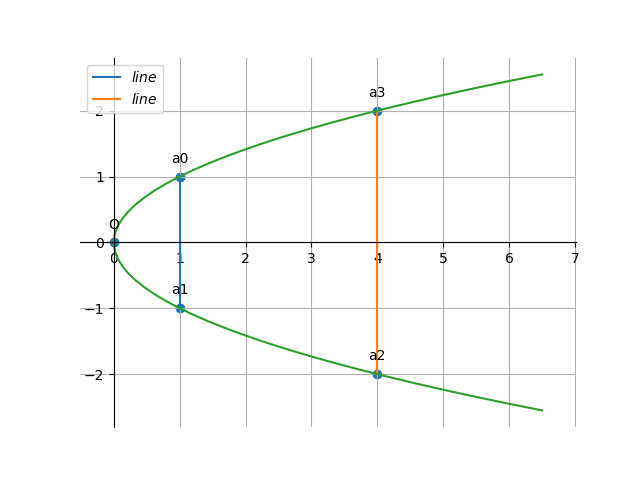
\includegraphics[width=0.75\columnwidth]{chapters/12/8/1/1/figs/conics1.png}
		\caption{}
		\label{fig:12/8/1/1}
  	\end{figure}

The parameters of the conic are
\begin{align}
	\vec{V} = \myvec{0 & 0\\0 & 1},
	\vec{u} = -\frac{1}{2}\myvec{ 1\\0},
	f = 0
	%\\
\end{align}
\iffalse
The point of intersection of the lines $x=1$ and $x=4$ to the parabola is given by


The points of intersection of the line 
\begin{align}
	L: \quad \vec{x} = \vec{q} + \kappa \vec{m} \quad \kappa \in \mathbf{R}
\label{eq:conic_tangent}
\end{align}
with the conic section are given by
\begin{align}
\vec{x}_i = \vec{q} + \kappa_i \vec{m}
\label{eq:conic_tangent_pts}
\end{align}
%
where
{\tiny
\begin{multline}
\kappa_i = \frac{1}
{
\vec{m}^T\vec{V}\vec{m}
}
\lbrak{-\vec{m}^T\brak{\vec{V}\vec{q}+\vec{u}}}
\\
\pm
\rbrak{\sqrt{
\sbrak{
\vec{m}^T\brak{\vec{V}\vec{q}+\vec{u}}
}^2
-
\brak
{
\vec{q}^T\vec{V}\vec{q} + 2\vec{u}^T\vec{q} +f
}
\brak{\vec{m}^T\vec{V}\vec{m}}
}
}
\label{eq:tangent_roots}
\end{multline}
}
\fi
For the line $x-1=0$, the parameters are  
\begin{align}
	\vec{q}_2=\myvec{1\\0},
	\vec{m}_2=\myvec{0\\1}
\end{align}
Substituting from the above in 
\eqref{eq:tangent_roots},
\begin{align}
\kappa_i=1,-1
\end{align}
yilelding 
the points of intersection 
\begin{align}
	\vec{a}_0=\myvec{1\\1},
	\vec{a}_1=\myvec{1\\-1}
\end{align}
Similarly, 
for the line $x-4=0$ 
\begin{align}
\vec{q_1}=\myvec{4\\0},
\vec{m_1}=\myvec{0\\1}
\end{align}
yielding
\begin{align}
\kappa_i=2,-2
\end{align}
from which, the points of 
intersection are
\begin{align}
\vec{a_3}=\myvec{4\\2},
\vec{a_2}=\myvec{4\\-2}
\end{align}
		See \figref{fig:12/8/1/1}.
Thus, 
the area of the parabola in between the lines $x=1$ and $x=4$ is given by
\begin{align}
\int_{0}^{4} \ \sqrt{x} \,dx-\int_{0}^{1} \ \sqrt{x} \,dx
=14/3
\end{align}
